\section{Experiment and Analysis}
\label{sec:experimentdesign}

To study spectrum utility in multiple populated areas, we develop experiments on off-the-shelf 
wireless platform and remote controlled spectrum analyzer measurement platform.
We do measurements in typical populated areas and sparse areas of DFW metropolitan 
carrying these platforms. According to the measured data, we apply our Multiband 
Access Points Estimation framework to analyze the performance of white space 
bands application in network deployment.

\subsection{Experiment Design}
% Platform
To ensure the results are applicable, we employ a Linux-based 802.11 testbed~\cite{Gateworks}.
The platform includes a Gateworks 2358 board with Ubiquiti XR radios (XR9 at 900 MHz, 
XR2 at 2.4 GHz, XR5 at 5.2 GHz) and a DoodleLabs DL475 radio at 450 MHz~\cite{Ubnt,Gateworks}.
We developed shell script with tcpdump for this testbed working as a sniffer recording all 
802.11 packets.
We perform experiments in downtown Dallas, SMU campus, neighborhood. The results show there
 is no 802.11 packets detected in white space bands(450 MHz, 900 MHz). And in DFW area, as 
 far as we know, we are the only group holds FCC license of white space bands. 
 Our experiments verify that these bands have not been used for commercial wireless data communication.
Moreover, we observed that Gateworks platform only update its received signal strength when received
a new packet. It is not good for inter-network interference measurement. To cover the gap, 
we employ a spectrum analyzer, multiband antenna, mobile antenna and a laptop developing 
a spectrum sensing system. 

% Data normalize 
As far as we know, there is no mobile multiband antenna in the market. We carry 700 MHz
mobile antenna in the middle of white space bands perform the outdoor experiments. 
Then, we uniform the mobile antenna 
measurements across bands comparing with the measurements from multiband antenna in 
lab with our controlled signal source. First we use USRP(Universal Software Radio Peripheral) 
N210 generate signals in 450 MHz, 800MHz, 2.4 GHz~\cite{usrp}. We feed the USRP 
signals directly to a spectrum analyzer and adjust configuration of USRP making 
the received signal strength the same as 5.2 GHz signal from Gatework 2358 with 
a XR5 radio. Then we connect the signal sources to the multiband antenna, measure the 
received signal in a fixed distance with 700 MHz antenna and antennas fit for each bands
to get the antenna loss of all the bands. Then we normalize the received signal strength 
of measurements collected through 700 MHz mobile antenna.

  \begin{figure}
  %\vspace{-0.0in}
  \centering
  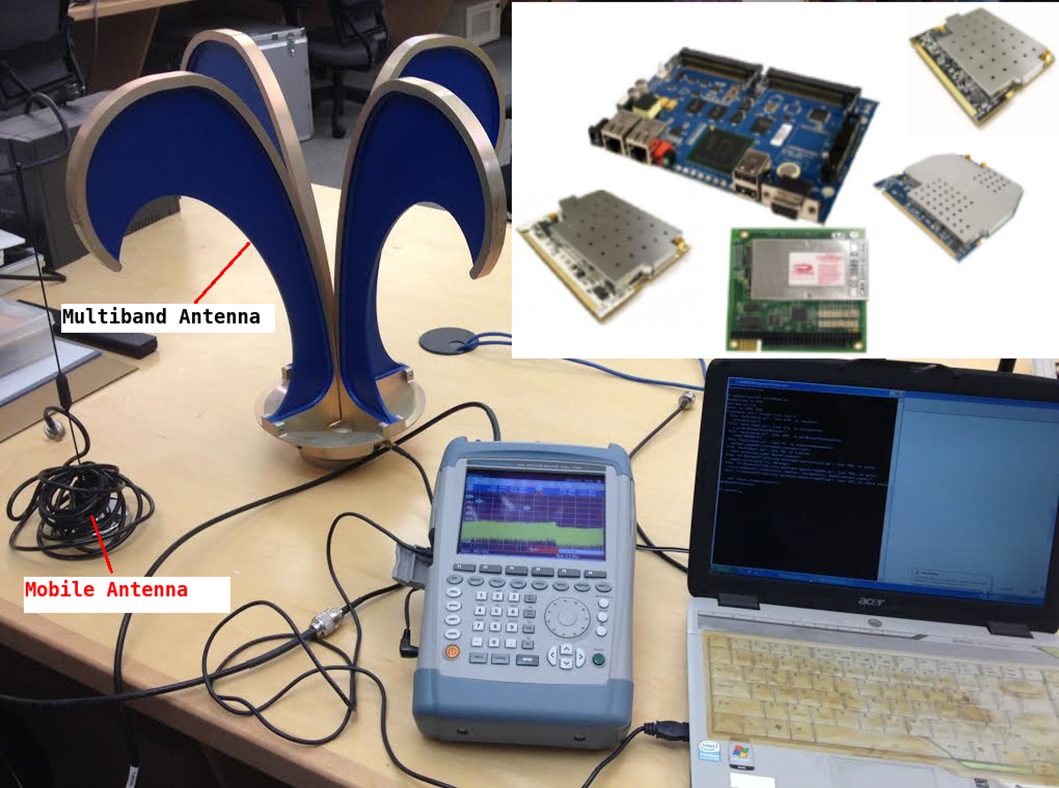
\includegraphics[width=74mm]{figures/equipment}
  \vspace{-0.1in}
  \caption{Multiband Measurement Platform}
  \label{fig:equipment}
  \vspace{-0.15in}
  \end{figure}
  
% Duplicate measurement in WiFi
Our experiment platforms are shown in Figure~\ref{fig:equipment}.
We have 32 samples each second from the spectrum analyzer system with a time stamp of all bands.
Gateworks sniffer platform record all the packets received in WiFi bands with time stamps. The duplicated 
samples in WiFi bands from spectrum analyzer and Gateworks are unique through the time stamp. 
Then we use the uniformed data for activity level calculation in WiFi bands. The activity level 
of white space bands rely on the spectrum analyzer measurements.  

% Location and Process 
%We apply drive test carrying our platform from Dallas to Weatherford as shown in~\ref{sec:problemformulation}.
We choose experiments locations according to population distribution in DFW metropolitan. 
The experiments are performed in Dallas, Weatherford and Millsap marked with stars in Figure~\ref{fig:drivemap}.
We have multiple measurements at neighborhood, campus and urban area in Dallas, our base.
In Weatherford and Millsap, we monitor wireless activities in 3 locations for 45 minutes in 
static on a normal weekday. Downtown, neighborhood and rural area are chosen from Weatherford and Millsap. 
Then we post-process these data getting the activity level of each band in all the location.


% Here
\subsection{Results and Analysis} 
\label{subsec:result}
In this subsection, we discuss our measurement results and perform our WAPE framework analyzing the 
influence of white space channels across diverse population densities.
In table~\ref{tab:activitymeasurement}, we show our measurement results in multiple locations of DFW metro.
Dallas as the central city of North Texas, has the highest activities in most of the measured bands,
 especially in 450 MHz. The measurements of Dallas urban are taken from SMU campus, 2 neighborhoods
 and city Plano. Our average these data, finding 2.4 GHz is more active in urban area rather than 
 downtown area. Most of schools campus and neighborhoods are covered by public or private WiFi today,
which brings more activities in 2.4 GHz and 5.2 GHz.
In Weatherford, all the bands have less activities than Dallas. And due to the measurement location
we have chosen, the rural area we chose on the west of Weatherford where could get more interference from
Fort Worth.
Millsap is a typical sparse city has 500 residents total in north Texas. The activities across all the bands are lower than
Dallas, and Weatherford. For 450 MHz, the activity reduces much faster than other bands in Dallas
and Weatherford. 

\begin{table*}
\centering % centering table 
\begin{tabular}{|l|c|c|c|c|c|c|c|c|c|c|c|} % creating 12 columns 
\hline %\hline % inserting double-line 
Bands     & \multicolumn{3}{c|}{Dallas} & \multicolumn{3}{c|}{Weatherford} & \multicolumn{3}{c|}{Millsap} \\% [0.5ex]
\hline % inserts single-line 
% Entering 1st row 
Area Type & Downtown & Urban & Sparse Area & Downtown &  Urban   & Sparse Area & Downtown & Urban & Sparse Area \\ % [0.5ex]
\hline % inserts single-line 
450 MHz &24.3667	&25.8274  &23.7667	&6.050 &12.50  &14.0333 & 7.0000 & 0.0667 & 0.0215 \\      
\hline % inserts single-line                                                                                                       
800 MHz &4.4000 	&16.4940  &4.7667	&5.2167&5.0667 &4.4333  & 3.8667 & 4.2000 & 3.6000 \\      
\hline % inserts single-line                                                                                                      
2.4 GHz &15.8667 	&34.9488  &2.6000	&2.0333&2.0333 &2.7667  & 2.0667 & 1.6000 & 0.8000 \\      
\hline % inserts single-line                                                                                                     
5.2 GHz &19.7000	&35.4571  &1.5333	&1.9333&1.9333 &1.3333  & 1.2667 & 2.0667 & 2.1000 \\      
\hline % inserts single-line 
\end{tabular}    
\label{tab:activitymeasurement}    
\caption{Activity Level in Multiple Locations} % title name of the table 
%\vspace{-0.4in}
\end{table*}    

We put these measuerment based activity level into our framework presented in~\ref{algorithm:mape}. We use Millsap
sparse area, Millsap downtown, Weatherford urban, Dallas urban, and Dallas downtown measurement as input activity level
map to the population density.
We input these information to our framework and calculate the number of access point for covering 
a $13 km \times 13 km$ area varying population density. The output is shown in Figure~\ref{fig:redensity}. 

   \begin{figure}
   %\vspace{-0.0in}
   \centering
   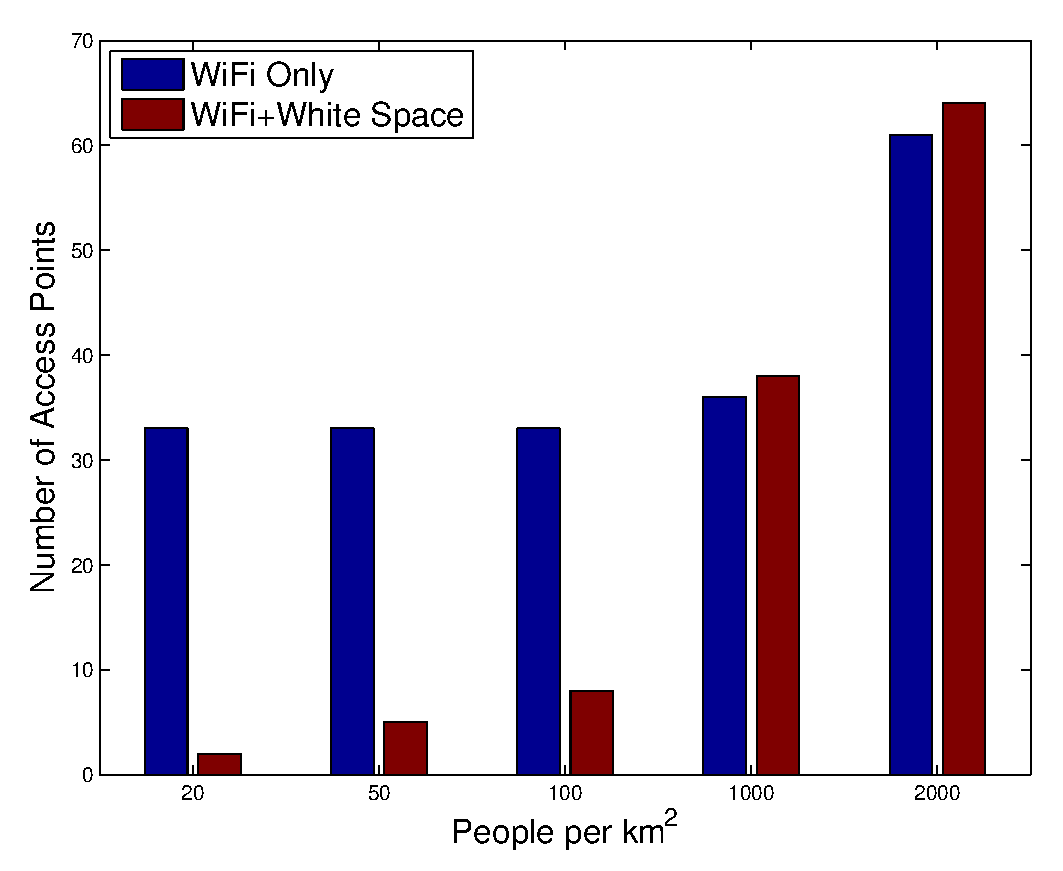
\includegraphics[width=74mm]{figures/redensity}
   \vspace{-0.1in}
   \caption{Number of Access Points need for 13x13 $km^2$ Area}
   \label{fig:redensity}
   \vspace{-0.1in}
   \end{figure}

% Experiment Results & expect results
In the calculation, we set the demand request as $2\ Mbps$ per person, the population
density as $20,50,100,1000,2000$ per square kilometers. We assume $30\%$ residents will use this
service, the maximum transmit power $30 dBm$, path loss exponent $3.5$~\cite{meikle2012global}. 
For WiFi only, we use 6 channels in 2.4 GHz, and 3 channels in 5.2 GHz. 
We adopt 802.11n maximum data rate 600 Mbps. For WiFi+ White Space
scenario, we use 3 channels in 450 MHz, 2.4 GHz and 5.2 GHz each. Then all the scenarios have the 
same channels in total. As shown in Figure~\ref{fig:redensity},
with the same number of channels, WiFi+White Space gains $1650\%$ comparing to WiFi only in 20 people 
per square kilometer scenario, and $660\%$ in 50 people per square kilometer and $412.5\%$ in 100 people
per square kilometer. But as the population density increase, due to the capacity constraint servicing
people in this area, low frequency white space band lose their advantage of larger communication range. 
And at the same time, the activities of other signal source, such as TV station in downtown area reduce
the capacity of white space band, then WiFi+White Space bands perform worse than WiFi only bands combination.
If we count the intra-network interference which is out of our scope, the situation could be even worse.
Moreover, FCC has stricter policy of white spaces in downtown and urban area. Fewer channels
are available in these area which make WiFi bands a better option for population dense areas.



To find the best bands combination, we select 500 people per square kilometer scenario and use Weatherford 
downtown spectrum to calculate the number of access points in this area. We assume the total number of channels 
is 12. The other setup of the experiment is 
the same as the previous configuration. The results are shown in~\ref{tab:500comb}.
 
 
 \begin{table}[h]
 \centering
 \begin{tabular}{|c|c|c|}
 \hline
 No. of Bands & Bands Combination & No. of AP & No. of AP \\
 \hline
 \multirow{4}{*}{One Band}    & 450 MHz  & 12  & 35 \\
 \cline{2-3}
                              & 800 MHz & 10  &  30 \\
 \cline{2-3}
			      & 2.4 GHz & 33  &  37 \\
 \cline{2-3}
                              & 5.2 GHz & 193 &  193 \\ 
 \hline
 \multirow{6}{*}{Two Bands}   & 450 MHz,800 MHz & 11  & 32\\
 \cline{2-3}
                              & 450 MHz,2.4 GHz & 23  & 36\\
 \cline{2-3}
			      & 450 MHz,5.2 GHz & 23  & 69\\
 \cline{2-3}
			      & 800 MHz,2.4 GHz & 20  & 33\\ 
 \cline{2-3}
			      & 800 MHz,5.2 GHz & 20  & 59\\ 
 \cline{2-3}
			      & 2.4 GHz,5.2 GHz & 33  & 73\\ 
 \hline
 \multirow{4}{*}{Three Bands} & 450 MHz,800 MHz,2.4 GHz & 16  & 33\\
 \cline{2-3}
                              & 450 MHz,800 MHz,5.2 GHz & 16  & 48\\
 \cline{2-3}
			      & 450 MHz,2.4 GHz,5.2 GHz & 33  & 53\\
 \cline{2-3}
			      & 800 MHz,2.4 GHz,5.2 GHz & 30 &  49\\ 
 \hline
 Four Bands & 450,800 MHz,2.4,5.2 GHz & 21  & 44 \\
 \hline
 \end{tabular}
 \caption{Channel Combinations for $500$ and $1500$ Population Density Scenarios}
 \label{tab:500comb}
 \end{table}



 
 
In the table, we compare the number of access points with 12 channels in all the possible combination of bands.
When all the channels are in the same band. as frequency goes up, more access points 
are need to serve the area. 450 MHz does not outperform 800 MHz in single band case because 
450 MHz channels have larger measured activity level in experiment setup.
White space band channels outperform wifi bands up to 1830\% in single band case.
Also we have equal channels in 2 bands shown in the table, the numerical results shows 
white space bands combination(450 MHz,800 MHz) performs better than WiFi only(2.4 GHz, 5.2 GHz) by 200\% and 
WiFi + white space bands(800 MHz, 2.4 GHz) by 81.8\%. In this population density, the more white space bands channels are 
used, the better performance will be got. White space channels bring 106.25\% in channels in 3 bands scenario.
And with 4 bands, the number of access points does not outperform using channels in white space bands.
Spreading channel distribution does not bring benefit for network deployment.

 \begin{table}[h]
 \centering
 \begin{tabular}{|l|p{3.5cm}|c|c|}
 \hline
 No. of Bands & Bands Combination & No. of AP & Min No. \\
 \hline
 \multirow{4}{*}{One Band}    & 450 MHz  & 35  & \multirow{4}{*}{30} \\
 \cline{2-3}
                              & 800 MHz & 30  &                      \\
 \cline{2-3}
							  & 2.4 GHz & 37  &                      \\
 \cline{2-3}
							  & 5.2 GHz & 193 &                      \\ 
 \hline
 \multirow{6}{*}{Two Bands}   & 450 MHz,800 MHz & 32  & \multirow{6}{*}{32} \\
 \cline{2-3}
                              & 450 MHz,2.4 GHz & 36  &                      \\
 \cline{2-3}
							  & 450 MHz,5.2 GHz & 69  &                      \\
 \cline{2-3}
							  & 800 MHz,2.4 GHz & 33  &                      \\ 
 \cline{2-3}
							  & 800 MHz,5.2 GHz & 59  &                      \\ 
 \cline{2-3}
							  & 2.4 GHz,5.2 GHz & 73  &                      \\ 
 \hline
 \multirow{4}{*}{Three Bands} & 450 MHz,800 MHz,2.4 GHz & 33  & \multirow{4}{*}{33} \\
 \cline{2-3}
                              & 450 MHz,800 MHz,5.2 GHz & 48  &                      \\
 \cline{2-3}
							  & 450 MHz,2.4 GHz,5.2 GHz & 53  &                      \\
 \cline{2-3}
							  & 800 MHz,2.4 GHz,5.2 GHz & 49 &                      \\ 
 \hline
 Four Bands & 450,800 MHz,2.4,5.2 GHz & 44  & 44 \\
 \hline
 \end{tabular}
 \caption{Bands Combinations of The Same No. of Channels in 500 Population Density}
 \label{tab:1500comb}
 \end{table}


We reset the population density as 1500. And Dallas urban spectrum activity is 
used in experiment shown in table\ref{tab:1500comb}.
In this scenario, all channels in one white space band still outperform WiFi 
combinations, but the maximum gain decreases to 543.33\%.
Compare to table~\ref{tab:500comb}, as population density increase, the gain brought by white space decrease. 
Generally adding white space band channels still has benefit reducing the number of access points
over WiFi only combination up to 128.12\%. 
The best
band combination is still the combination with white space bands. 

